\documentclass[a4paper,11pt,openany]{book}
\usepackage[utf8]{inputenc}
\usepackage{amsmath, amssymb}
\usepackage{graphicx}
\usepackage{hyperref}
\usepackage{subcaption}
\graphicspath{ {images/} }
\usepackage[dvipsnames]{xcolor}

% Book's title and subtitle
\title{\Huge \textbf{Mathematics behind}
 \\
 \Huge \textbf{ Engineering Drawing} \vspace{10pt}\\\huge{COP290 Project }}
% Author
\author{\textsc{Arpan Mangal}
 \\
 \textsc{Deepanshu Jindal}}

%\definecolor{indexColor}{rgb}{0.0742, 0.188, 0.2734}
\hypersetup{
  colorlinks   = true, %Colours links instead of ugly boxes
  urlcolor     = blue, %Colour for external hyperlinks
  linkcolor    = black,%brown, %191970, %Colour of internal links
  citecolor   = red %Colour of citations
}

\begin{document}

\frontmatter
\maketitle

\tableofcontents
%\listoffigures
%\listoftables

\mainmatter

\chapter{Introduction}

\indent Engineering Drawing is a vital part of Mechanical Engineering. Mechanical students are given extensive training in this subject which consists of taking orthographic projections of a given 3 Dimensional object and retrieving the object from its 2 Dimensional orthographic projections. \\
\indent The question is can this monotonous job be automated with the help of a computer. This report deals with developing a mathematical model to accomplish this task of automating the subject of Engineering Drawing.

\section{Terminology and conventions used for describing 3D Objects}
\indent This section deals with the terminology used in this book for describing the object and its orthographic projections. We will work with the third angle of projection. \\
\indent Consider a simple three dimensional object as in Fig. 1.1 below:
\begin{figure}[h]
\centering
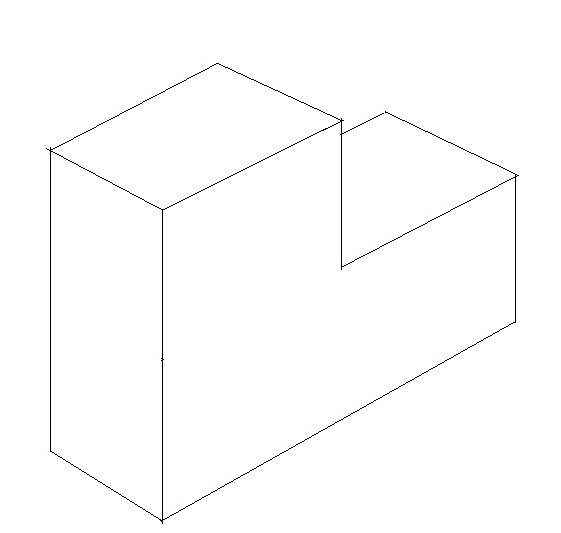
\includegraphics[scale=0.4]{obj}
\caption{A 3-Dimensional object}
\label{a3dObj}
\end{figure}
\\ \\
\indent We will see it in third angle of projection. For that we will assume that orientation of coordinate axes as follows:
\begin{figure}[!h]
\centering
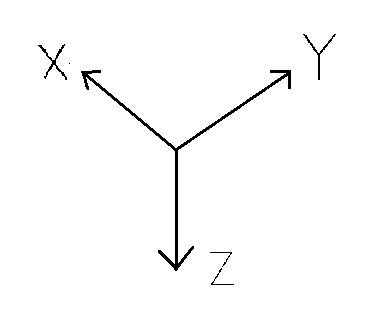
\includegraphics[scale=0.3]{direc}
\caption{Orientation of axes}
\end{figure}

\indent This is to say that the front view will lie on the Y-Z plane, top view on the X-Y plane and the side view on the Z-X plane. \\
\indent The orthographic projections will then be plotted onto the three planes as below:

\begin{figure}[h]
\centering
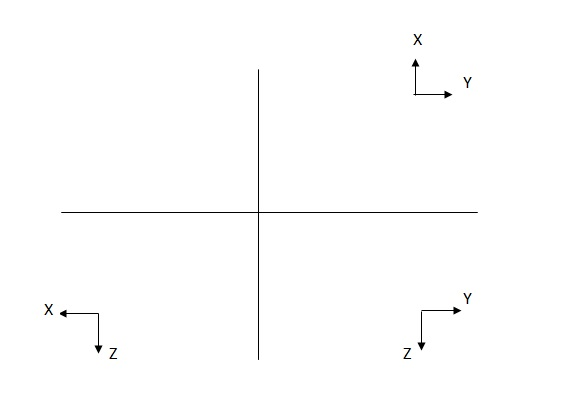
\includegraphics[scale=0.5]{2dLabels}
\caption{Terminology for specifying axes labels on the 3 planes}
\end{figure}

\begin{figure}[h]
\centering
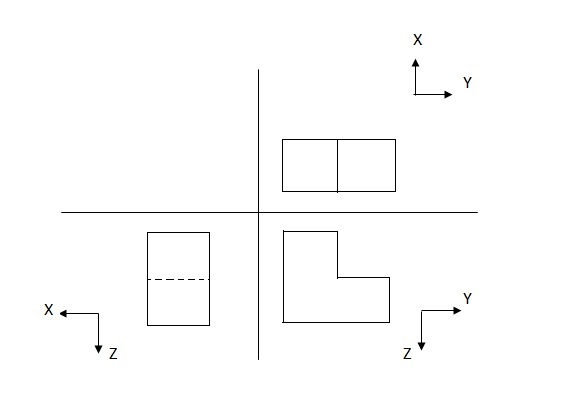
\includegraphics[scale=0.6]{2d}
\caption{Actual orthographic projections of the object}
\end{figure}

\vspace{10 mm}
\section{Package Features}
\indent This software will consist of mainly two features:
\begin{enumerate}
  \item Constructing orthographic projections from the given 3-Dimensional object.
  \item Re-construction of the 3-Dimensional object from given orthographic projections and constructing isometric view of the 3-D reconstruction.
\end{enumerate}

Each part has its own expected input and output as described below:

\subsection{Orthographic Projections from 3-D}
\indent  We will take a 3-dimensional graph, $G(V,E)$ as 
%, $G(V,E)$ as input from the user.
%various points $\boldsymbol{X_i}$'s and labeled
a set of 3 dimensional points $\boldsymbol{X_i}$'s as input along with the set of corresponding labelled edges $\boldsymbol{L_i}$'s between them. 

The output shall consist of the three orthographic projections on the three orthographic planes as shown in Fig. 1.3. The user can also specify an arbitrary plane along which we can construct the auxiliary view of the object.

\subsection{Re-construction of 3-D object from its orthographic projections}
We will take the three orthographic projections from the user as shown in Fig. 1.3. Each projection will be set of points $\boldsymbol{X_i}$'s along with the connecting lines. Each point will consist of a label which will remain same across the three projections for the corresponding point.

Output shall be a 3-D plot and an isometric projection of the reconstructed object.

% End Introduction

\chapter{Generating Projections of 3D Models}

\indent This chapter deals with projecting 3-dimensional models and figures to a 2-dimensional surface. This includes projection on the three Cartesian planes as well as any given cutting plane. We will take $3^{rd}$ angle of projection.\\
\indent We will proceed by projecting points, lines and finally complete models which consists of lines and points.

\section{Projection of a single point}

This section describes projecting single point in 3D to a 2D surface. We will consider that we are given a point, $\boldsymbol{P}$ in the form of a vector:

% Useful sources:
    % http://www.sas.rochester.edu/psc/thestarlab/help/latextut4.pdf
    % https://tex.stackexchange.com/questions/69997/how-to-write-an-m%E2%A8%89n-matrix-in-latex
    
\begin{equation}
P = 
\left(\begin{array}{c} X_i \\ Y_i \\ Z_i\end{array}\right) 
\end{equation}
    
We will show that projection of the point on any plane can be obtained simply by multiplying suitably chosen matrix $\boldsymbol{M}$ with the vector $\boldsymbol{P}$ . 
\subsection{Projecting on one of the Cartesian planes}
We have three Cartesian planes: X-Y, Y-Z and Z-X. We will project the point in each of the three planes. \\
\indent Consider the projection of $\boldsymbol{P}$ on X-Y plane. It would simply be equivalent to dropping the z-coordinate and keeping the x and y coordinates intact, i.e. the projection $\boldsymbol{p_{xy}}$ of $\boldsymbol{P}$ would be: 

\begin{equation}
p_{xy} = 
\left(\begin{array}{c} X_i \\ Y_i \end{array}\right) 
\end{equation} \\

This could be written as:

\begin{equation}
p_{xy} = 
\left(\begin{array}{c} x_i \\ y_i \end{array}\right) =
\left(\begin{array}{ccc} 1 & 0 & 0 \\ 0 & 1 & 0 \end{array}\right) 
\left(\begin{array}{c} X_i \\ Y_i \\ Z_i\end{array}\right) 
\end{equation}

or,

\begin{equation}
p_{xy} = 
\left(\begin{array}{ccc} 1 & 0 & 0 \\ 0 & 1 & 0 \end{array}\right)P
\end{equation}

Similarly,

\begin{equation}
p_{yz} = 
\left(\begin{array}{ccc} 0 & 1 & 0 \\ 0 & 0 & 1 \end{array}\right)P
\end{equation}

and,

\begin{equation}
p_{zx} = 
\left(\begin{array}{ccc} 0 & 0 & 1 \\ 1 & 0 & 0 \end{array}\right)P
\end{equation}

Equations 2.4 through 2.6 describe the projection of point $\boldsymbol{P}$ on the three Cartesian planes.

\subsection{Projection on an arbitrary plane surface}
Any arbitrary plane surface,  $\boldsymbol{\Pi}$, can be represented by the position of its origin, $\boldsymbol{O'}$ and the direction of its axes $\boldsymbol{X'}$, $\boldsymbol{Y'}$, and $\boldsymbol{Z'}$ w.r.t. the original axes. (Here $\boldsymbol{Z'}$ is the normal to the plane  $\boldsymbol{\Pi}$, and  $\boldsymbol{X'}$ \&  $\boldsymbol{Y'}$ form the plane surface)\\

First, lets consider translation only i.e. shifting of origin with fixed direction of coordinate axes. Suppose, the shifted origin is at point $(\boldsymbol{X_o},\boldsymbol{Y_o},\boldsymbol{Z_o})$.
Then the new coordinated for point $\boldsymbol{P}$ shall be 
\begin{equation}
P' = 
\left(\begin{array}{c} X_i \\ Y_i \\ Z_i\end{array}\right) - \left(\begin{array}{c} X_o \\ Y_o \\ Z_o\end{array}\right)
= \left(\begin{array}{c} X_i-X_o \\ Y_i-Y_o \\ Z_i-Z_o\end{array}\right) = P - O'
\end{equation}
\\
\\Now, consider that the coordinate axes are rotated without translation.\\ Let the rotated coordinated axes be $\boldsymbol{X'}$, $\boldsymbol{Y'}$, and $\boldsymbol{Z'}$\\
\begin{figure}
\centering
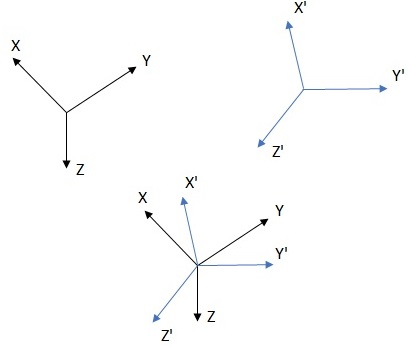
\includegraphics[scale=0.6]{rotation}
\caption{Rotation of Coordinate Axes}
\end{figure}
Let the unit vectors corresponding to $\boldsymbol{X'}$, $\boldsymbol{Y'}$, and $\boldsymbol{Z'}$ (w.r.t. old Cartesian coordinates $\boldsymbol{X}$, $\boldsymbol{Y}$, and $\boldsymbol{Z}$)respectively be 


\begin{equation}
\left(\begin{array}{c} \alpha_1 \\ \beta_1 \\ \gamma_1\end{array}\right),\left(\begin{array}{c} \alpha_2 \\ \beta_2 \\ \gamma_2\end{array}\right),
\left(\begin{array}{c} \alpha_3 \\ \beta_3 \\ \gamma_3\end{array}\right)
\end{equation}\\

The new coordinates of $\boldsymbol{P}$ can be obtained by multiplying with transformation matrix\footnote{Details about finding rotational transformation matrix in the Appendix} as
\begin{equation}
P' =
\left(\begin{array}{ccc} \alpha_1 & \beta_1 & \gamma_1 \\ \alpha_2 & \beta_2 & \gamma_2 \\ \alpha_3 & \beta_3 & \gamma_3 \end{array}\right) \left(\begin{array}{c} X_i \\ Y_i \\ Z_i\end{array}\right)
\end{equation}\\
or,
\begin{equation}
P' = RP
\end{equation}

Now, to consider any arbitrary plane we need to take into account both translation and rotation. Thus,
\begin{equation}
P' = R(P-O')
\end{equation}

Now the projection of the point $\boldsymbol{P}$ on this plane will be 
\begin{equation}
p' = \left(\begin{array}{ccc} 1 & 0 & 0 \\ 0 & 1 & 0 \end{array}\right)R(P-O')
\end{equation}\\


\section{Projection of a Line}
A line can be uniquely determined using two distinct points lying on it (say $\boldsymbol{P_{1}}$ and $\boldsymbol{P_{2}}$). 
\\
We will represent the line as a 3 x 2 matrix represented as ($\boldsymbol{P_{1}}$,  $\boldsymbol{P_{2}}$)
\begin{equation}
L = 
\left(\begin{array}{cc} X_1 & X_2 \\ Y_1 & Y_2 \\ Z_1 & Z_2\end{array}\right) 
\end{equation}
As seen in section 2.1, projection of a single point can be obtained by multiplication of point vector by suitable matrix. Now, the projection of line on the plane will be same as a line drawn on the plane joining the projections of the points.
\subsection{Projecting on one of the Cartesian planes}
\begin{equation}
L_{xy} = \left(\begin{array}{c c} x_1 & x_2\\ y_1 & y_2 \end{array}\right) =
\left(\begin{array}{ccc} 1 & 0 & 0 \\ 0 & 1 & 0 \end{array}\right) 
\left(\begin{array}{cc} X_1 & X_2 \\ Y_1 & Y_2 \\ Z_1 & Z_2\end{array}\right)
\end{equation}
or,

\begin{equation}
L_{xy} = 
\left(\begin{array}{ccc} 1 & 0 & 0 \\ 0 & 1 & 0 \end{array}\right)L
\end{equation}

Similarly,

\begin{equation}
L_{yz} = 
\left(\begin{array}{ccc} 0 & 1 & 0 \\ 0 & 0 & 1 \end{array}\right)L
\end{equation}

and,

\begin{equation}
L_{zx} = 
\left(\begin{array}{ccc} 0 & 0 & 1 \\ 1 & 0 & 0 \end{array}\right)L
\end{equation}

\subsection{Projection on an arbitrary plane surface}
Just as we derived for the case of projection of point on arbitrary plane $\boldsymbol{\Pi}$, similarly the projection of the line, $\boldsymbol{L}$ on the $\boldsymbol{X'-Y'}$ plane will be given by:
\begin{equation}
L'_p = 
\left(\begin{array}{ccc} 1 & 0 & 0 \\ 0 & 1 & 0 \end{array}\right)R(L-O')
\end{equation}

\indent (Here $\boldsymbol{O'}$ $\equiv$ ($\boldsymbol{O'}$, $\boldsymbol{O'}$))

\section{Projection of 3D Models}
For representational purposes a 3D model can be thought of as a set of lines making up the edges and planes making up the faces. By projecting all the edges and all the faces we would be able to obtain the projection of the entire object.

A set of bounding edges would define a plane. Thus if we are able to project the edges, then their projections shall give us the projection of plane bounded by these edges. 

\subsection{Spatial arrangement of planes and hidden lines}
With the naive implementation of the procedure stated above we can develop a projection drawing by considering the 3D object as a wireframe, however with that we would lose out on the information about spatial orientation of plane and hidden lines in the drawing.

To know which plane lies above others we need to follow a procedure in selecting the order in which points are projected.

Firstly, we arrange the points in order of decreasing distance from the plane of projection. We start projecting points onto the plane in this order.

As soon as both of the points defining an edge are projected on the plane we join the on the projection making up the projection of edge.
We continue doing this process. As soon as all the lines bounding a plane are projected, we know that the topmost plane has been projected. Now any edge projected thereafter which pass through this plane will have to be a hidden edge.\footnote{Details about finding that a point lies within a polygon in appendix}

We keep adding points, edges and planes in this order and we can be sure that all the visible parts are projected on the plane first and any edges added thereafter which pass through a plane has to be a hidden edge.

\chapter{3D Reconstruction from projections}
This chapter deals with creating the 3-dimensional reconstruction of an object given its three (or atleast two) orthographic projection. We will also see about the existence and uniqueness of the solution.

We will proceed as before, first reconstructing points, then lines and finally 3D objects.

\section{Reconstruction of a single point from given orthographic projection}
Let us take a single point $\boldsymbol{P_i}$ shown in each of the three projections. 

\begin{figure}[h]
\centering
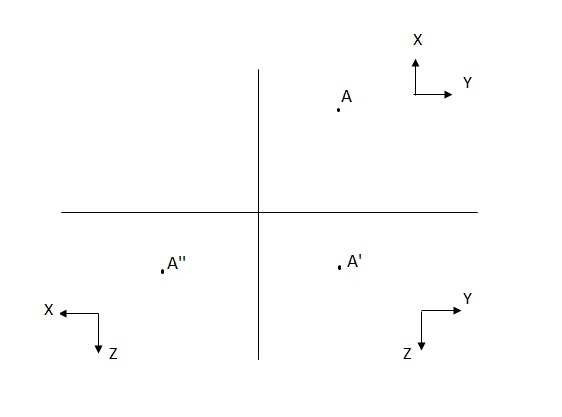
\includegraphics[scale=0.5]{2dLabelswithPoint}
\caption{Projections of single point}
\end{figure}


The actual point in 3D will be of the form:

\begin{equation}
P_{i} = 
\left(\begin{array}{c} X_i \\ Y_i \\ Z_i \end{array}\right)
\end{equation}
 and its corresponding projections in the three planes would be:

XY Plane:
\begin{equation}
p = 
\left(\begin{array}{c} x_i \\ y_i\end{array}\right)
\end{equation}

YZ Plane:
\begin{equation}
p' = 
\left(\begin{array}{c} y_i' \\ z_i'\end{array}\right)
\end{equation}

ZX Plane:
\begin{equation}
p'' = 
\left(\begin{array}{c} z_i'' \\ x_i''\end{array}\right)
\end{equation}


Using the method of projecting 3D point in 2D as in 2.1,
\begin{equation}
p = 
\left(\begin{array}{ccc} 1 & 0 & 0\\ 0 & 1 & 0\end{array}\right)P
\end{equation}
\begin{equation}
p' = 
\left(\begin{array}{ccc} 0 & 1 & 0\\ 0 & 0 & 1\end{array}\right)P
\end{equation}
\begin{equation}
p'' = 
\left(\begin{array}{ccc} 0 & 0 & 1\\ 1 & 0 & 0\end{array}\right)P
\end{equation}

resulting in the equation,
\begin{equation}
\left(\begin{array}{c} x_i \\ y_i \\ y_i' \\ z_i' \\ z_i'' \\ x_i'' \end{array}\right) = 
\left(\begin{array}{ccc} 1 & 0 & 0\\ 0 & 1 & 0\\ 0 & 1 & 0\\ 0 & 0 & 1\\ 0 & 0 & 1\\ 1 & 0 & 0 \end{array}\right)P
\end{equation}


Now, for existence of a solution \\
 $x_i = x_i'', y_i = y_i', z_i' = z_i',$\footnote{If not then the given orthographic projections are incompatible and hence a reconstruction is not possible.}.

This gives,
\begin{equation}
\left(\begin{array}{c} x_i \\ y_i \\ y_i \\ z_i \\ z_i \\ x_i \end{array}\right) = 
\left(\begin{array}{ccc} 1 & 0 & 0\\ 0 & 1 & 0\\ 0 & 1 & 0\\ 0 & 0 & 1\\ 0 & 0 & 1\\ 1 & 0 & 0 \end{array}\right)P
\end{equation}


Removing redundant rows,
\begin{equation}
\left(\begin{array}{c} x_i \\ y_i \\ z_i \end{array}\right) = 
\left(\begin{array}{ccc} 1 & 0 & 0\\ 0 & 1 & 0\\ 0 & 0 & 1 \end{array}\right)P
\end{equation}

This has unique solution namely,
\begin{equation}
\left(\begin{array}{c} X_i \\ Y_i \\ Z_i \end{array}\right) =
\left(\begin{array}{c} x_i \\ y_i \\ z_i \end{array}\right)
\end{equation}

which is the required point in 3D.

Clearly, for projection of a single point we need only the three coordinates for which two orthographic projections are both necessary and sufficient.

\section{Reconstruction of a line}
Let us take a single line $\boldsymbol{L_i}$ joined by points $\boldsymbol{A_i}$ and $\boldsymbol{B_i}$.

\noindent In the three projections it will correspond to three lines 
\begin{equation}
l_i \equiv (a_i, b_i) , l_i' \equiv (a_i', b_i') , l_i'' \equiv (a_i'', b_i'')
\end{equation}

If the line is normal to a Cartesian plane then, in the corresponding orthographic projection, the points  $\boldsymbol{A_i}$ and $\boldsymbol{B_i}$ shall be coinciding.

We will use the same method as defined above in section 3.1 to derive the points

\begin{equation}
A_i =
\left(\begin{array}{c} A_{i\_x} \\ A_{i\_y} \\ A_{i\_z} \end{array}\right)
\end{equation}
and,
\begin{equation}
B_i =
\left(\begin{array}{c} B_{i\_x} \\ B_{i\_y} \\ B_{i\_z} \end{array}\right)
\end{equation}.

Our line, $\boldsymbol{L_i}$ will then be $\boldsymbol{L_i \equiv (A_i, B_i)}$. 

\section{Reconstructing a wire frame of a 3D object}
Let us consider a 3-Dimensional object as shown in Fig. 3.2 . It will consist of lines $\boldsymbol{L_i}$'s and points $\boldsymbol{P_i}$'s.
\begin{figure}[h]
\centering
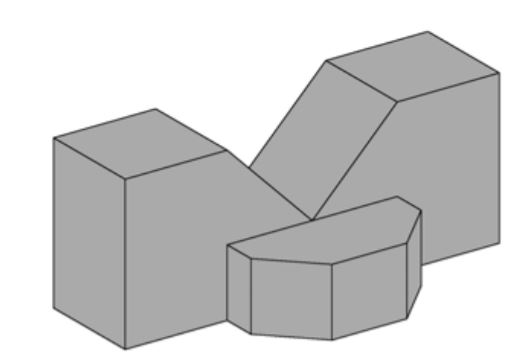
\includegraphics[scale=0.3]{3DModel}
\caption{A 3-D Object}
\end{figure}


We will be given its three orthographic projections as shown in Fig. 3.3 and we will assume that we are given point correspondence in each view i.e., for a point $\boldsymbol{p_i}$ in a view, corresponding points $\boldsymbol{p_i'}$ and $\boldsymbol{p_i''}$ are shown in the two other views.

\begin{figure}[h]
\centering
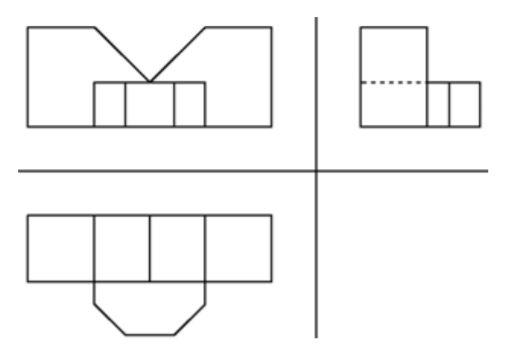
\includegraphics[scale=0.6]{OrthographicProjections}
\caption{Orthographic Projections of the object ($1^{st}$ angle)}
\end{figure}


Further we are given various $\boldsymbol{l_i}$'s in the three orthographic projections. The lines given to us may not be exhaustive and could pose several problems. This is discussed in the following section.

\subsection{Intermediate vertices and collinear edges}

Consider a orthographic projection as below:
\begin{figure}[h]
\centering
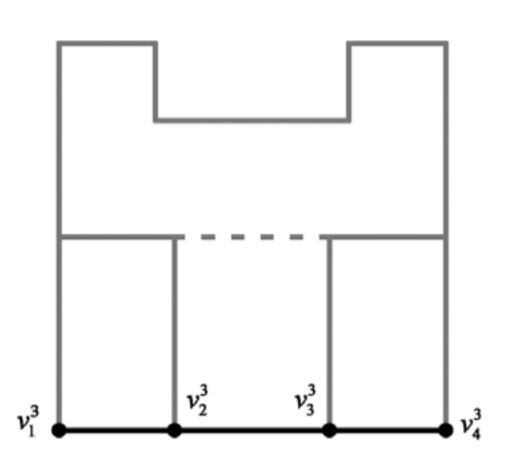
\includegraphics[scale=0.5]{ProjectedView}
\caption{A projected view}
\end{figure}

Consider the lowest line. This line consist of many edges, for ex. $v_1v_2$, $v_2v_4$, $v_1v_4$ etc. Now we do not expect the user to enter each of the possible permutations. The user will input either $v_1v_4$ or combinations like $v_1v_2$ and $v_2v_4$.

First we will follow a method called segmentation. In this for each edge we will iteratively check for all the possible existence of intermediate vertices. If no intermediate vertex is found, the procedure stops. Otherwise the found intermediate
vertex causes the creation of two new edges (unless one of them
already exists). We will perform this for each set of edges belonging to a projection, thus adding new edges to our edge set.

This is depicted in Fig. 3.5. 

\begin{figure}[ht]
\centering
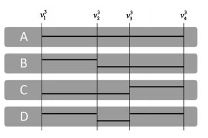
\includegraphics[scale=0.9]{possibleCombinationEdges}
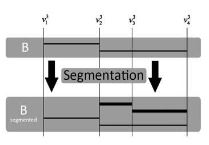
\includegraphics[scale=0.9]{Segmentation}
\caption{Segmentation procedure for creating additional edges}
\end{figure}

This segmentation task will create additional short edges out of larger edges like $v_1v_4$ but still it may not be exhaustive. For ex. say it may divide $v_1v_4$ into $v_1v_2$ and $v_2v_4$, the latter being further subdivided. It will leave out permutations such as $v_1v_3$. 

So after the segmentation task, a check of collinearity of edges is performed. This is fundamental when two non contiguous vertices are linked by two or more edge all collinear one with each other. This procedure will add new edges like $v_1v_3$ to our set of edges.

This is depicted in Fig. 3.6 .
\begin{figure}[ht]
\centering
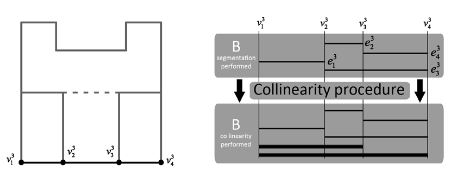
\includegraphics[scale=0.9]{Collinearity}
\caption{Collinearity procedure for creating additional edges}
\end{figure}

After performing these two procedures we will get a set of edges, $\boldsymbol{E_i}$ for each of the three projections (i is the label for the three planes). Each of the set will contain edges/lines $\boldsymbol{l_j}$ joined by some points $\boldsymbol{a_i}$ and $\boldsymbol{b_i}$. From the three sets so obtained we will remove out all the edges which conflict in the orthographic projections. (A non conflicting relationship exists if there exist a line between the two points in all the three projections or the points are coincident in one of the projection. )

On the remaining edges we will follow the same procedure for lines as detailed in section 3.2 . This would give us the corresponding points $\boldsymbol{A}$ and $\boldsymbol{B}$ in 3-D which join to form our line $\boldsymbol{L}$.


\begin{figure}[ht]
\centering
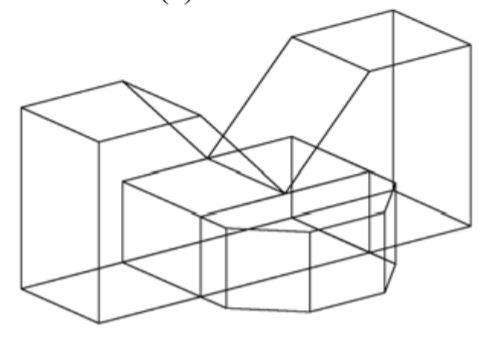
\includegraphics[scale=0.5]{PseudoWireFrame}
\caption{Pseudo-Wire frame of re-constructed object}
\end{figure}

The set of points $\boldsymbol{P}$ and edges $\boldsymbol{E}$ in 3-D constructed in this manner will give us our reconstruction of the object in the form of a wireframe model. It will be a wireframe model of the true 3-D object similar to that shown in Fig. 3.7. However this wireframe may contain some extra connecting lines between two points which should not be there. We will call this a "pseudo wireframe".\\

We need to remove these extra edges to obtain the real object's wireframe as shown in Fig. 3.8. 

\begin{figure}[ht]
\centering
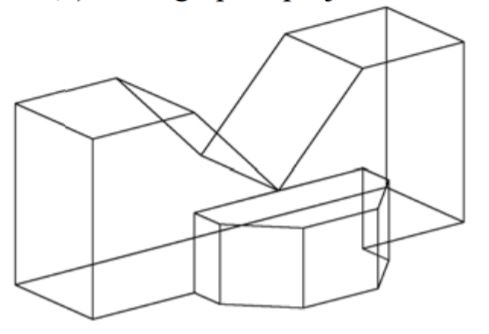
\includegraphics[scale=0.5]{WireframeModel}
\caption{Wire frame of re-constructed object}
\end{figure}

It is for sure that no actual line will be left out because for every line $\boldsymbol{L_i}$ there will correspond a line $\boldsymbol{l_i}$ in each of the three views whether solid or hidden, from which our algorithm will infer an actual line $\boldsymbol{L_i}$ in 3-D. 

\subsection{Removing extra edges from Pseudo-wireframe}
Many of the false edges and features derived from the drawing can be removed by following what is knows as \textbf{Pruning Strategy} derived by \textit{Markovsky et al}.

According to this strategy keep iterating over the following four steps until no feature is removed in a loop:
\begin{enumerate}
  \item A vertex lying on just one or no edges is removed, together with that edge.
  \item A vertex lying on just two collinear edges is removed and the two edges are replaced by a single edge.
  \item Three or more edges meeting at a vertex where all of the edges are coplanar, are removed unless they have a collinear extension.
  \item A vertex lying on just two non-collinear edges is removed together with those edges.
\end{enumerate}

This \textbf{Pruning Strategy} shall remove the false features from the wireframe giving us the desired wireframe reconstruction of the 3D object. 

\subsection{Rotation of the Wireframe}
Rotation of the wireframe obtained for observation by the user can be carried out by multiplying with rotation transformation matrix as illustrated in sections 2.1.2 and 2.2.2.


% End 3-D Reconstruction

\chapter{Representing 3D Models in Isometric View }
Isometric projection is a method for visually representing three-dimensional objects in two dimensions.


\begin{figure}[h]
 \centering
\begin{subfigure}{0.4\textwidth}
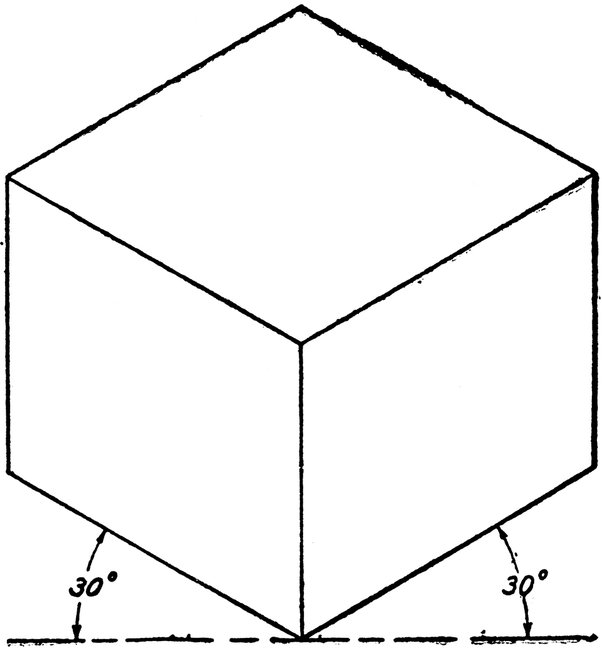
\includegraphics[scale=0.2]{isometric2} 
\caption{Isometric drawing for a cube}
\label{fig:subim1}
\end{subfigure}
\begin{subfigure}{0.4\textwidth}

\includegraphics[scale=0.23]{isometric}
\caption{Isometric graph}
\label{fig:subim2}
\end{subfigure}
 
\caption{Isometric representation}
\label{fig:image2}
\end{figure}

Isometric view can be obtained for a 3D object by suitable rotations followed by dimension reduction.The object is first rotated around the vertical axis by $45^{\circ}$ followed by a rotation about horizontal axis by $35.264^{\circ}$.

The isometric transform from a point $A$ in 3D space to a point $b$ in 2D space looking into the first octant can be obtained as:
\begin{equation}
\left(\begin{array}{c} b_x \\ b_y \\ 0 \end{array}\right) = \left(\begin{array}{ccc} 1 & 0 & 0 \\ 0 & 1 & 0 \\ 0 & 0 & 0 \end{array}\right)\left(\begin{array}{ccc} 1 & 0 & 0 \\ 0 & cos \alpha & sin \alpha \\ 0 & -sin \alpha & cos \alpha \end{array}\right)\left(\begin{array}{ccc} cos \beta & 0 & -sin \beta \\ 0 & 1 & 0 \\ sin \beta & 0 & cos \beta \end{array}\right)\left(\begin{array}{c} A_x  \\ A_y \\ A_z \end{array}\right)
\end{equation}
where $\alpha$ = $35.264^{\circ}$ and $\beta$ = $45^{\circ}$\\

or, 
\begin{equation}
b = \frac{1}{\sqrt[]{6}}\left(\begin{array}{c} \sqrt[]{3}A_x - \sqrt[]{3}A_z \\ A_x + 2A_y + A_z \end{array}\right)
\end{equation}\\

To find the isometric projections for the edges, we just have to project the corresponding endpoints of an edge, and by drawing a line between them we will obtain the projection of the edge.

Thus given coordinates for vertices and edges for any 3D solid, we can obtain its isometric projection using the above given formula. For obtaining isometric projection from different octants we just have to multiply the point coordinates with a suitably chosen rotational transformation matrix.
\appendix
\chapter{Rotational Transformation Matrix}
We look into the problem of finding a rotational transformation matrix when an arbitrary rotated plane is specified 
\subsection{When plane is specified as a point lying on it and normal vector}
We consider any arbitrary line passing through not parallel to normal. \\
Taking cross product of this line with normal(say $\vec{n}$) will give us a vector which lies perpendicular to the normal vector and hence lies on the plane. We normalise this obtained vector to get a unit vector(say $\vec{p}$) lying in the plane.
Now taking a cross product of $\vec{n}$ and $\vec{p}$ will give us another unit vector $\vec{q}$ lying in plane orthogonal to $\vec{p}$.

Now together $\vec{p}$,$\vec{q}$ and $\vec{n}$ for a new orthogonal system for coordinates.
Let these vectors with respect to the Cartesian coordinate system be represented as :

\begin{equation}
\left(\begin{array}{c} p_1 \\ p_2 \\ p_3\end{array}\right),
\left(\begin{array}{c} q_1 \\ q_2 \\ q_3\end{array}\right) and
\left(\begin{array}{c} n_1 \\ n_2 \\ n_3\end{array}\right)
\end{equation} \\

The rotation transformation matrix for transforming coordinates 

\begin{equation}
\left(\begin{array}{ccc} p_1 & p_2 & p_3 \\ q_1 & q_2 & q_3 \\ n_1 & n_3 & n_3 \end{array}\right) 
\end{equation}

\subsection{When plane is specified as a set of point lying on it }
For unique determination of a plane we need atleast three no collinear points. Let $P_1$, $P_2$ and $P_3$ be three such points on plane.
Then, we consider two vectors namely $\boldsymbol{P_1P_2}$ and $\boldsymbol{P_1P_3}$. Now taking a cross product of the two gives us the normal vector $\vec{n}$ of the plane. \\
Also normalising $\boldsymbol{P_1P_2}$ gives us a vector lying on plane $\vec{p}$. 
Now taking its crossproduct with $\vec{n}$ and continuing as above gives us the required rotation tranformation matrix.

\chapter{Point inside a polygon}
This section addresses the problem of determining whether a point lies inside the polygon or not.

Firstly, if the coordinate of point lie beyond the extreme coordinates of the polygons, then we can be sure that the point is outside the polygon. If this is not the case, then we must do something else. We will use an algorithm known as \textbf{ray casting}. The idea of the algorithm is pretty simple: Draw a virtual ray from anywhere outside the polygon to the point under consideration and count how often it hits a side of the polygon. If the number of hits is even, it's outside of the polygon, if it's odd, it's inside.
\begin{figure}[!h]
\centering
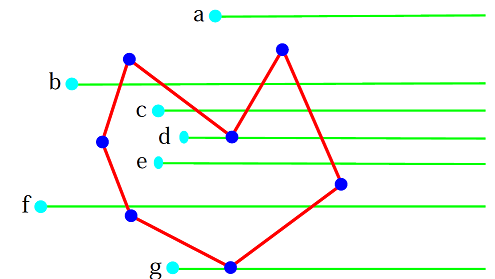
\includegraphics[scale=0.8]{polygon}
\caption{Ray Casting}
\end{figure}

The special cases such as that for the point \textbf{g} in the above figure, or the case when an edge is coincident with the casted ray, we need to handle things differently.

If a point lies on the casted ray then we can either add both the edges sharing that point as a hit or ignore them altogether, since the parity remains same in both the case.

If an edge is coincident with the casted ray then we must ignore that edge. The edges adjacent to this edge can either both be counted or left out, again due to indifference to the parity caused by this.

% bibliography
\begin{thebibliography}{9}
\bibitem{2Dto3D}
From 2D Orthographic views to 3D Pseudo-Wireframe: An Automatic Procedure
\url{http://www.ijcaonline.org/volume5/number6/pxc3871296.pdf}

\bibitem{2Dto3D}
\href{https://books.google.co.in/books?id=zw-6_p9WUnIC&pg=PA284&lpg=PA284&dq=Removal+of+extra+edges+from+a+wireframe+algorithm&source=bl&ots=Njj7ljww6_&sig=eZoa8eT-TWU_4RVm0A1qTl6RrGk&hl=en&sa=X&ved=0ahUKEwij5JqzienYAhXBNI8KHVGOCZAQ6AEIKDAA#v=onepage&q=Removal}{Graphics Recognition: Algorithms and Systems}
\textit{Karl Tombre}
\bibitem{isometric}
  \url{https://en.wikipedia.org/wiki/Isometric_projection#Mathematics}
  
\bibitem{PointinPolygon}
\url{https://stackoverflow.com/questions/217578/how-can-i-determine-whether-a-2d-point-is-within-a-polygon}



\end{thebibliography}

\end{document}


